% This work is made available under the terms of the
% Creative Commons Attribution-ShareAlike 4.0 license,
% http://creativecommons.org/licenses/by-sa/4.0/.
%
% Version: $Revision$

\documentclass[a4paper]{book}

\usepackage{wrapfig}
\usepackage{graphicx}
\usepackage{hyperref}
\usepackage{multirow}
\usepackage{scalefnt}
\usepackage{tikz}

% watermark -- for draft stage
%\usepackage[firstpage]{draftwatermark}
%\SetWatermarkLightness{0.9}
%\SetWatermarkScale{5}

% Copyright (c) 2009 by the University of Waikato, Hamilton, NZ. 
% This work is made available under the terms of the 
% Creative Commons Attribution-ShareAlike 4.0 license,
% http://creativecommons.org/licenses/by-sa/4.0/.
%
% Version: $Revision: 2916 $

\newenvironment{tight_itemize}{
\begin{itemize}
  \setlength{\itemsep}{1pt}
  \setlength{\parskip}{0pt}
  \setlength{\parsep}{0pt}}{\end{itemize}
}

\newenvironment{tight_enumerate}{
\begin{enumerate}
  \setlength{\itemsep}{1pt}
  \setlength{\parskip}{0pt}
  \setlength{\parsep}{0pt}}{\end{enumerate}
}

% if you just need a simple heading
% Usage:
%   \heading{the text of the heading}
\newcommand{\heading}[1]{
  \vspace{0.3cm} \noindent \textbf{#1} \newline
}

\newcommand{\icon}[1]{\tikz[baseline=-3pt]\node[inner sep=0pt,outer sep=0pt]{\includegraphics[height=1.1em]{#1}};}


\title{
  \textbf{ADAMS} \\
  {\Large \textbf{A}dvanced \textbf{D}ata mining \textbf{A}nd \textbf{M}achine
  learning \textbf{S}ystem} \\
  {\Large Module: adams-weka-webservice} \\
  \vspace{1cm}
  
\includegraphics[width=5cm]{images/weka-webservice-module.png} \\
}
\author{
  Peter Reutemann \\
  Michael Fowke
}

\setcounter{secnumdepth}{3}
\setcounter{tocdepth}{3}

\begin{document}

\begin{titlepage}
\maketitle

\thispagestyle{empty}
\center
\begin{table}[b]
	\begin{tabular}{c l l}
		\parbox[c][2cm]{2cm}{\copyright 2012-2017} &
		\parbox[c][2cm]{5cm}{
\includegraphics[width=5cm]{images/coat_of_arms.pdf}}
	\end{tabular}
	
\includegraphics[width=12cm]{images/cc.png} \\
\end{table}

\end{titlepage}

\tableofcontents
\listoffigures
%\listoftables

%%%%%%%%%%%%%%%%%%%%%%%%%%%%%%%%%%%
\chapter{Set up}
The default set up for the webservice is to run on the local machine, or
\textit{localhost}. If you want to publish the webservice, either within
a LAN or over the internet, then you need to update the URL and/or port that the 
webservice binds to and is available for clients.

\section{Client}
If you use ADAMS clients, you need to change the WSDL for the WEKA webservice
to point the clients to the right address. You can find the WSDL for the 
webservice at the following location:
\begin{verbatim}
  resources/wsdl/weka/WekaService.wsdl
\end{verbatim}
In this file, change the \textit{location} attribute of the \textit{soap:address} 
tag appropriately. For instance, from this:\
\begin{verbatim}
  <soap:address location="http://localhost:9090/WekaServicePort"/>
\end{verbatim}
to this:
\begin{verbatim}
  <soap:address location="http://weka.blah.com:8080/WekaServicePort"/>
\end{verbatim}

\begin{figure}[htb]
  \centering
  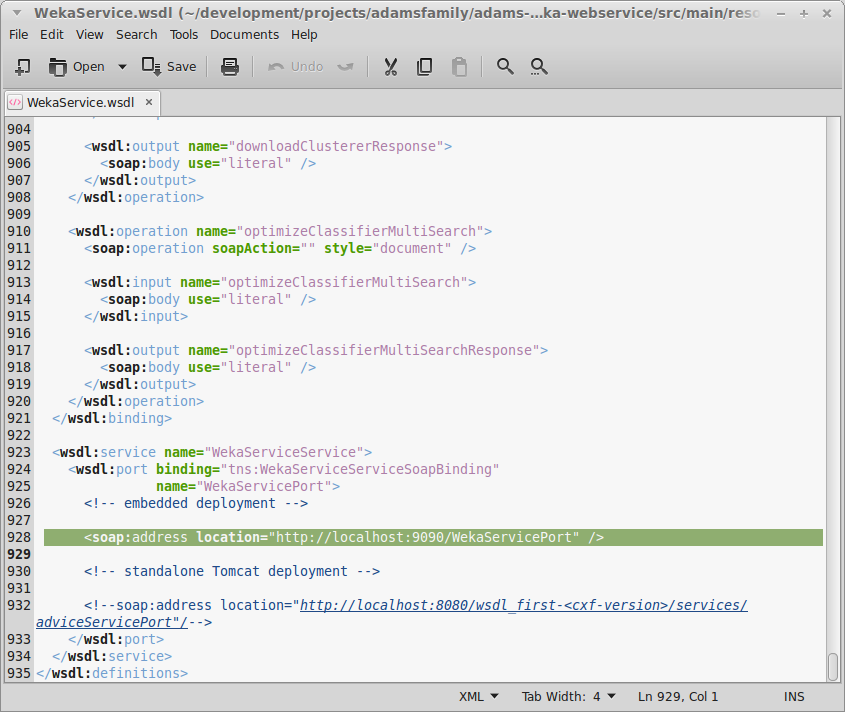
\includegraphics[width=10.0cm]{images/client_setup.png}
  \caption{Tag in the WSDL to change for the clients.}
  \label{client_setup}
\end{figure}

\clearpage
\section{Server}
In addition to the changes to the WSDL as described in the section on the 
\textit{Client}, the server requires another modification
when launched from the flow. In case of the example server 
workflow\footnote{adams-weka-webservice-weka-webservice.flow},
you can do this by changing the \textit{URL} property located here:
\begin{tight_itemize}
	\item \textit{WSServer} actor
	\item \textit{webService} property
	\item \textit{URL} property
\end{tight_itemize}
For instance, if the server's running the webservice is \textit{weka.blah.com}
and is supposed to use port 8080, then use the URL 
\textit{http://weka.blah.com:8080/WekaServicePort}. 

\textbf{NB:} Ensure that the port is not blocked by a firewall running on the server
or already used otherwise.

\begin{figure}[htb]
  \centering
  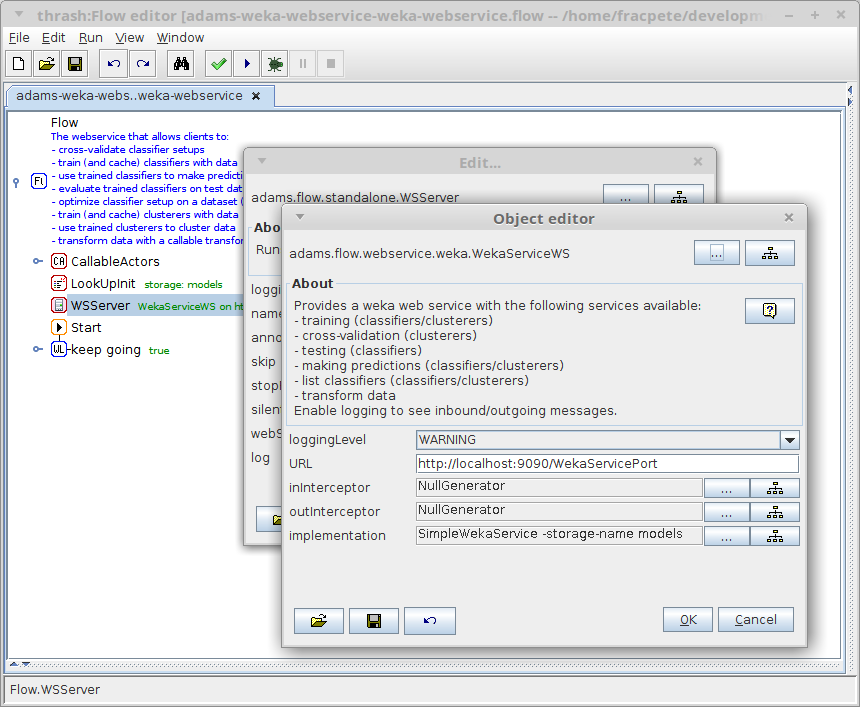
\includegraphics[width=10.0cm]{images/server_setup.png}
  \caption{Displaying dialog with URL the webservice binds to.}
  \label{server_setup}
\end{figure}

\clearpage
\chapter{Usage}
Before you can use the webservice, you need to start the server side. You can
do this by simply starting the example server 
flow\footnote{adams-weka-webservice-weka-webservice.flow}.

\section{Classifiers}
The webservice offers the following functionality for classifiers:
\begin{tight_itemize}
	\item \textit{cross-validation} -- cross-validates a specified classifier
	setup on a provided dataset and returns the statistics.\footnote{adams-weka-webservice-crossvalidate-classifier.flow}
	\item \textit{train} -- trains a classifier setup on a provided dataset 
	and stores the model for future use in a lookup table in internal
	storage.\footnote{adams-weka-webservice-train-classifier.flow}
	\item \textit{test} -- evaluates a stored model with a new dataset and
	returns the statistics.\footnote{adams-weka-webservice-test-classifier.flow}
	\item \textit{predict} -- uses a stored model to generate predictions for
	a provided dataset.\footnote{adams-weka-webservice-predict-classifier.flow}
	\item \textit{list} -- lists all the names of the currently stored classifier
	models.\footnote{adams-weka-webservice-list-classifiers.flow}
	\item \textit{display} -- returns the string representation of a stored
	classifier model.\footnote{adams-weka-webservice-display-classifier.flow}
	\item \textit{download} -- downloads a previously trained a classifier 
	model.\footnote{adams-weka-webservice-download-classifier.flow}
	\item \textit{optimize} -- performs parameter-optimization for a classifier
	using a dataset, for an arbitrary number of search parameter settings using 
	the \texttt{weka.classifiers.meta.MultiSearch} meta-classifier. The best setup is 
	then returned.\footnote{adams-weka-webservice-optimize-classifier-multi-search.flow}
\end{tight_itemize}

\section{Clusterers}
The webservice offers the following functionality for clusterers:
\begin{tight_itemize}
	\item \textit{train} -- trains a clusterer setup on a provided dataset 
	and stores the model for future use in a lookup table in internal
	storage.\footnote{adams-weka-webservice-train-clusterer.flow}
	\item \textit{predict} -- uses a stored model to predict cluster membership
	for	a provided dataset.\footnote{adams-weka-webservice-predict-clusterer.flow}
	\item \textit{list} -- lists all the names of the currently stored clusterer
	models.\footnote{adams-weka-webservice-list-clusterers.flow}
	\item \textit{display} -- returns the string representation of a stored
	clusterer model.\footnote{adams-weka-webservice-display-clusterer.flow}
	\item \textit{download} -- downloads a previously trained a clusterer 
	model.\footnote{adams-weka-webservice-download-clusterer.flow}
\end{tight_itemize}

\section{Filters}
The webservice also allows you to transform datasets using WEKA filters. This
works by providing a dataset and the name of the callable actor on the server.
You can define an arbitrary number of callable actors that transform datasets.
The only requirement is that they accept a \textit{weka.core.Instances} object
and generate such one as well.\footnote{adams-weka-webservice-transform.flow}

\begin{figure}[htb]
  \centering
  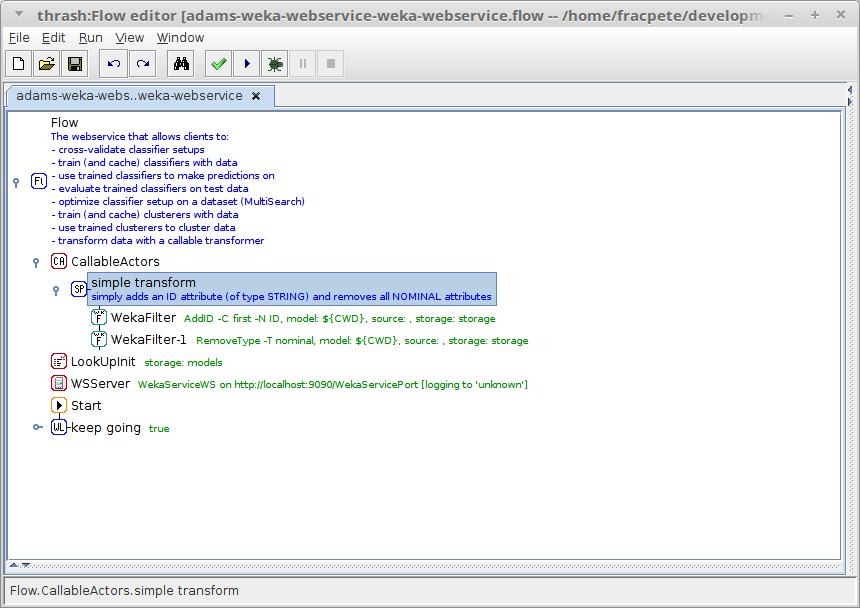
\includegraphics[width=10.0cm]{images/transform_callable_actor.png}
  \caption{Callable actor for transforming datasets.}
  \label{transform_callable_actor}
\end{figure}

\chapter{Development}
The default webservice implementation, \texttt{adams.flow.webservice.weka.SimpleWekaService},
is a very simply version providing the functionality. All processing happens
in a single thread. If you require a version that scales better and can handle
more and concurrent requests, then you might want to implement your own
backend. This is quite simple, as you only need to create a class that implements
the following interfaces:
\begin{tight_itemize}
	\item \texttt{nz.ac.waikato.adams.webservice.weka.WekaService}
	\item \texttt{adams.flow.webservice.weka.OwnedByWekaServiceWS}
\end{tight_itemize}
Or, you can simply subclass \texttt{adams.flow.webservice.weka.SimpleWekaService}
and override the method that needs your attention.

The class needs to be placed in the following package:
\begin{verbatim}
  adams.flow.webservice.weka
\end{verbatim}

%%%%%%%%%%%%%%%%%%%%%%%%%%%%%%%%%%%
% Copyright (c) 2009-2012 by the University of Waikato, Hamilton, NZ. 
% This work is made available under the terms of the 
% Creative Commons Attribution-ShareAlike 4.0 license,
% http://creativecommons.org/licenses/by-sa/4.0/.
%
% Version: $Revision: 3353 $

\begin{thebibliography}{999}
	% to make the bibliography appear in the TOC
	\addcontentsline{toc}{chapter}{Bibliography}

    % references
	\bibitem{adams}
		\textit{ADAMS} -- Advanced Data mining and Machine learning System \\
		\url{https://adams.cms.waikato.ac.nz/}{}

	\bibitem{imagemagick}
		\textit{ImageMagick} -- Software suite to Convert, Edit, and Compose Images \\
		\url{http://www.imagemagick.org/}{}

\end{thebibliography}


\end{document}
